\chapter{Model Validations}

So far, the validation has been done only for the results from one-stage experiment. Verification of the parameters identified in the two-stage experiment could not be performed since identification of the friction still have some problems that need to be solved. 

\section{Results Verification from One-stage Experiment}

After identifying the paramaters for all the required equation, developed algorithm model now was built to estimate the contact force. Hence, there are two versions of algortithm, one that use Dahl and another one that use coulomb and viscous. The estimated force is then compared to real force from F/T sensor for validation. The results are shown in \fref{fig:validation}.

\begin{figure}[H]
  \begin{subfigure}[t]{0.5\textwidth}
    \centering
    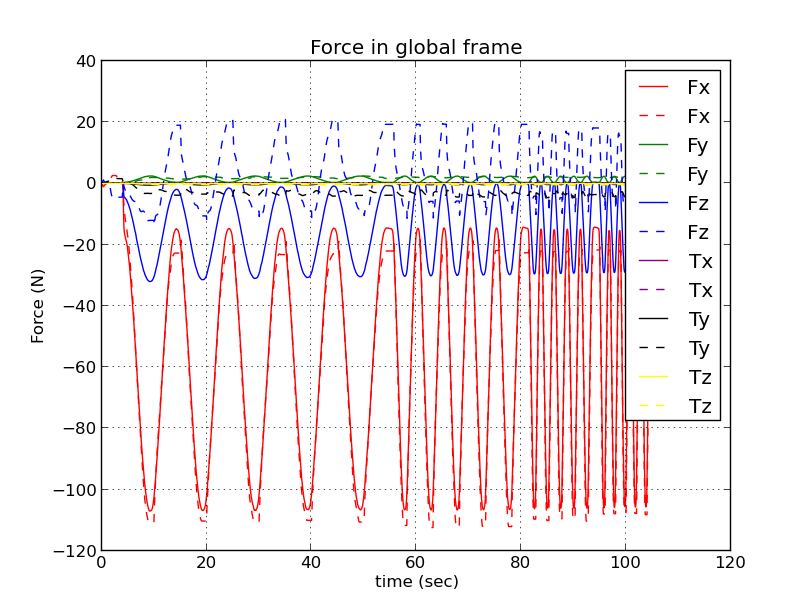
\includegraphics[width = \textwidth ]{fig14} 
    \caption{Using static model}
    \label{fig:static validation}
  \end{subfigure}
  \begin{subfigure}[t]{0.5\textwidth}
    \centering
    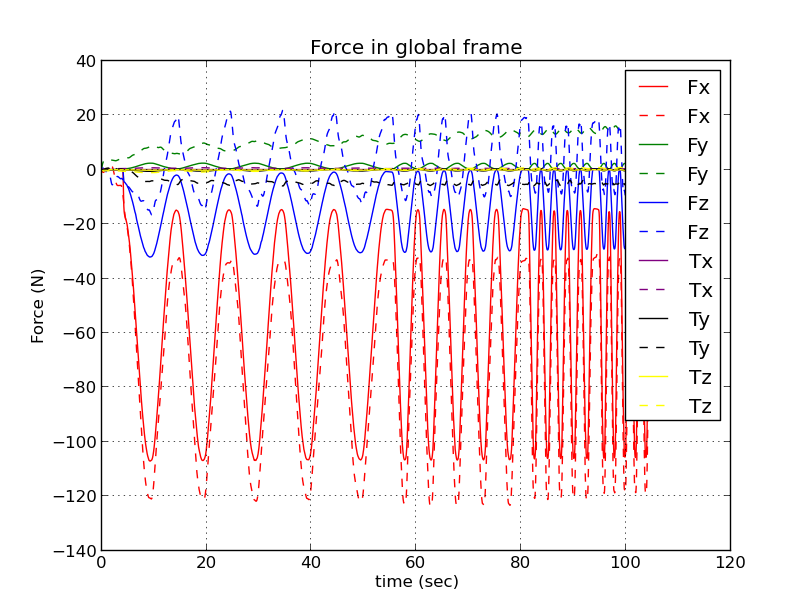
\includegraphics[width = \textwidth ]{fig15}
    \caption{Using Dahl model}
    \label{fig:Dahl validation}
  \end{subfigure}
  \caption{Validation result of estimated force. (- - : estimated output, -- : real output)}
  \label{fig:validation}
\end{figure}

\begin{figure}[H]
  \begin{subfigure}[t]{0.5\textwidth}
    \centering
    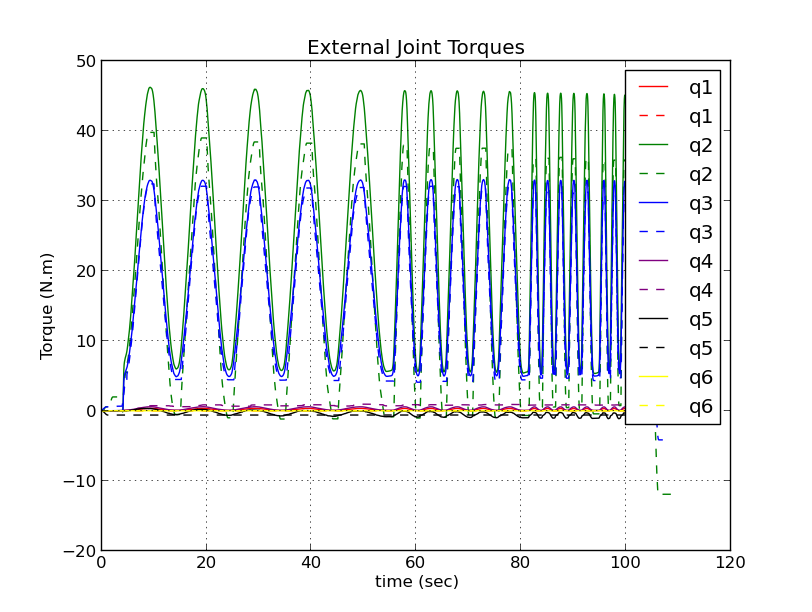
\includegraphics[width = \textwidth ]{fig16} 
    \caption{Using static model}
    \label{fig:static tor}
  \end{subfigure}
  \begin{subfigure}[t]{0.5\textwidth}
    \centering
    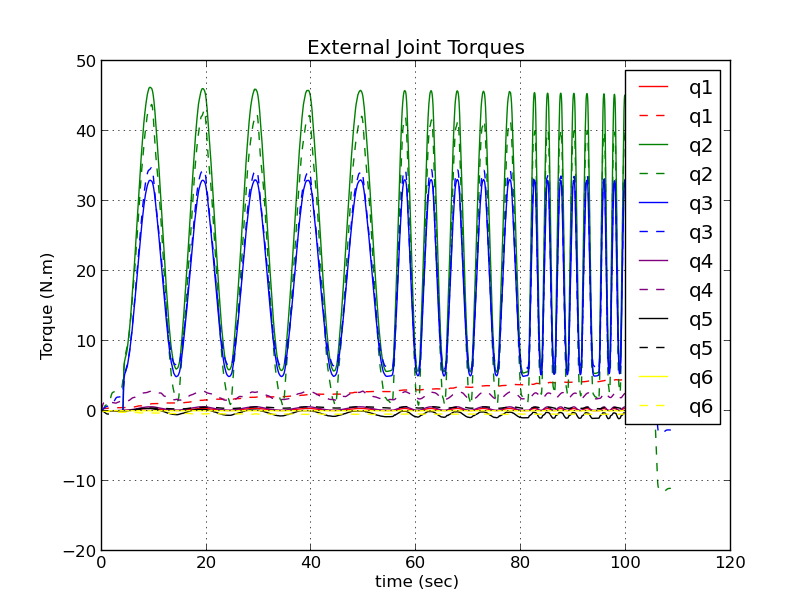
\includegraphics[width = \textwidth ]{fig17}
    \caption{Using Dahl model}
    \label{fig:Dahl tor}
  \end{subfigure}
  \caption{External joint torques estimation of \fref{fig:static validation} (- - : estimated output, -- : real output)}
  \label{fig:torque validation}
\end{figure}

In \fref{fig:Dahl tor} it is quite clear that Dahl algorithm gives a good estimation for second and third joint. However, it is bad when estimating the first joint. This is more likely due to two reasons. First, the initial state of $z$ might be incorrect. For every arm position, it is supposed to have specific state of $z$, however as we lack of knowledge of this value, it was only calculated using some basic assumption. The second reason is due to stability of motor currents. Since change of internal state is a function of rate of motor currents, unstable motor currents will drift the value of $z$. However, seeing that the value of first joint seems drifted over time, hence it is more likely that the second reason is the main problem. Due to this problems, it is then decided to leave the Dahl model for the rest of the progress.

On the other hand, the results using coulomb and viscous can be seen in \fref{fig:static validation} and \fref{fig:static tor}. The estimated force in x-axis is quite satisfactory and this is the main force that acting on the robot. However, the force estimation of other axis is not as good as the first one. This is because of the error estimation of external joint torques that leads to the force. The comparison of external joint torques estimation can be seen in \fref{fig:torque validation}. The root mean square error values of estimated contact force and torque using this model are presented in \tref{table:rmse}. On some aspects, especially for torques it has large errors. This is because there is no contact torques introduced, hence the value from force sensor is always near 0.

\begin{table}
    \centering
    \begin{tabular}{| c | c | c | c |}
    \hline
              & RMSE & max-min & RMSE / (max-min)(\%) \\ \hline
    Force x   & 5.231976  & 107.774842  & 4.854543  \\ \hline
    Force y   & 0.942644  & 2.391211    & 39.421205  \\ \hline
    Force z   & 18.686503 & 32.631091   & 57.265945  \\ \hline
    Torque x  & 0.116993  & 0.048434    & 241.550320  \\ \hline
    Torque y  & 3.542738  & 0.879940    & 402.611434  \\ \hline
    Torque z  & 0.350672  & 0.192694    & 181.983440  \\ \hline
    \end{tabular}
    \caption{Root mean square value of estimated contact force using static friction}
    \label{table:rmse}
\end{table}

While it gives a reasonable results for both model, this is partially because the old data was being used for validation, hence it is quite obvious that it will give a good estimation. Validation with new data will be required to really verify the developed model. 
